%\documentclass[journal=jacsat]{achemso}

\documentclass[10pt,aps,prl,twocolumn,amsmath,amssymb,superscriptaddress,longbibliography]{revtex4-1}

%\documentclass[preprint,showpacs,preprintnumbers,amsmath,amssymb]{revtex4-1}
%\documentclass[twocolumn,showpacs,preprintnumbers,amsmath,amssymb]{revtex4}
% Some other (several out of many) possibilities
%\documentclass[preprint,aps]{revtex4}
%\documentclass[preprint,aps,draft]{revtex4}
%\documentclass[prb,amsmath,amssymb]{revtex4}% Physical Review B

\usepackage{graphicx}% Include figure files
\usepackage{dcolumn}% Align table columns on decimal point
\usepackage{bm}% bold math
\usepackage{amsmath}% bold math
\usepackage{siunitx}% si units
\usepackage{color}
\usepackage{graphicx}
%\usepackage[normalem]{ulem}
%\nofiles

\bibliographystyle{achemso}
%\bibliographystyle{naturemag}
%\bibliographystyle{abbrv}

\begin{document}

\title{
Low-cost linear-scaling \emph{ab initio} molecular dynamics for weakly-interacting systems
}

\author{Hayden Scheiber}
\email{hayden.scheiber@mcgill.ca}
\author{Yifei Shi}
\author{Rustam Z. Khaliullin}
\email{rustam.khaliullin@mcgill.ca}
\affiliation{Department of Chemistry, McGill University, 801 Sherbrooke St. West, Montreal, QC H3A 0B8, Canada}

\date{\today}

\begin{abstract}
Linear scaling density functional theory based on absolutely localized molecular orbitals is used in conjunction with the Langevin equation of motion to create a low-cost molecular dynamics method for weakly coupled molecular systems which retains sufficient accuracy to generate correct dynamical properties in water. 

The approach utilizes a systematically inaccurate linear-scaling potential energy surface (PES) calculation method. 
Inaccuracies in the calculation of force using this method are balanced by a weighted version of the Langevin Equation of motion. 
The stochastic ``white noise'' of the Langevin Equation acts to smooth out PES discontinuities while also thermostating the system to maintain a constant thermodynamic temperature. 
We show that Langevin dynamics can be successfully implemented to reduce computational cost by allowing systematic error in PES calculation to be absorbed into the stochastic and damping forces associated with the Langevin equation. 
We also introduce a simple heuristic approach to find the best Langevin Equation parameters to use for balancing system-specific imperfect forces and maintaining correct dynamical behavior.
\end{abstract}

\maketitle
\section{Introduction}
Since the unification of molecular dynamics (MD) and density functional theory (DFT) in 1985 by Car and Parrinello,~\cite{a:thecpmd} much research has been focused on reducing the computational overhead of \emph{ab initio} molecular dynamics (AIMD) potential energy calculations.~\cite{b:aimd} 
% Remove Following text for some journals
AIMD provides a great advantage over traditional predefined-potential molecular dynamics in that it calculates its potential energy surface (PES) on-the-fly, rather than needing to be laboriously optimized to the specific system of interest beforehand. 
This allows for exploration of much more chemically complex systems than are possible with traditional MD methods. 
AIMD also allows for much greater predictive capability than traditional MD, as a first principles approach is not confined to a predetermined range of system parameters. 
The tradeoff is the computational complexity involved in calculating an accurate set of forces for each atom at every time step of the simulation.~\cite{a:2gen-cpmd}
% End remove

The computational cost of the straightforward approach to Kohn-Sham DFT is known to grow (or \emph{scale}) cubically with system size because it involves either diagonalization of the effective Kohn-Sham Hamiltonian or, if the direct optimization of Kohn-Sham orbitals is performed, the equally costly inversion of a preconditioner.~\cite{a:ot} % Add other references here?
This cubic scaling severely constricts the possible length and time scales accessible by AIMD using such an approach. 
In an attempt to address this issue, there has been much research into the possibility of linear scaling (LS) DFT methods for the calculation of forces.

% Most methods are based on localization of electrons into small sub domains of the system, so that long range charge transfer is ignored.~\cite{a:linscale3,a:lee-yang-1996,a:ls-scuseria-1997,a:ls-manolopoulos-1998,a:ls-helgaker-2001,a:ls-niklasson-2003,a:curvy2,a:ls-dm-sign,a:ls-parinello} So far the available methods still suffer from a high computational cost prefactor, even though they scale linearly for large systems. This has limited the available time scales for LS AIMD severely.

% Re-write the following section and include any recent advances
A number of such alternative methods explore the natural sparsity of the one-electron density matrix (DM)~\cite{a:ls-kohn-1996,a:ls-rev-1999} and are capable of yielding LS for large systems.~\cite{a:linscale3,a:lee-yang-1996,a:ls-scuseria-1997,a:ls-manolopoulos-1998,a:ls-helgaker-2001,a:ls-niklasson-2003,a:curvy2,a:ls-dm-sign} 
Unfortunately, the variational optimization of the DM is very inefficient for accurate DFT calculations,~\cite{a:ls-rev-1999,a:ls-dm-sign} which require many basis functions per atom. 
Therefore, the applications of DM-based LS methods have been limited to minimal-basis tight-binding problems. 
The optimal basis variants of the DM methods~\cite{a:ls-stechel-1994,a:ls-gillan-1995,a:ls-gillan-1996,a:ls-onetep-2003} designed to address this issue contract the large basis set into a small number of new localized basis functions and then optimize the DM in the contracted basis. 
Although such methods have been successfully used for the evaluation of accurate DFT energies of very large systems~\cite{a:ls-onetep-2009,a:ls-conquest-2010,a:ls-onetep-2010-app1,a:ls-rev-2012} their application for AIMD is hampered by the computationally costly optimization of both the contracted orbitals and the density matrix.
%
From this point of view, methods based on the direct optimization of localized KS orbitals~\cite{a:ls-galli-parrinello-1992,a:ls-mauri-galli-car-1993,a:ls-ordejon-1993,a:ls-mauri-galli-1994,a:ls-ordejon-1995,a:ls-kim-mauri-galli-1995,a:ls-fattebert-2004,a:ls-fattebert-2006,a:burger-yang-2008} are advantageous since they require only the occupied orbitals and, thus, deal with fewer variational degrees of freedom than the DM methods. 
Unfortunately, the progress in the development of orbital-based LS methods has been hindered by the inherently difficult convergence of the localized-orbital optimization.~\cite{a:ls-mauri-galli-car-1993,a:ls-ordejon-1995,a:ls-fattebert-2004,a:ls-rev-1999,a:weitao-yang-2013} 
%Furthermore, numerous proposed LS functionals exhibit multiple local minima, which limits their applicability in molecular dynamics simulations because of the resulting poor conservation of the total energy~\cite{a:ls-rev-1999}.

Hence, the computational prefactor of the existing LS DFT methods~\cite{a:ls-rev-1995,a:ls-rev-1999,a:ls-rev-2002,a:ls-rev-2012} remains very high and most AIMD simulations are still performed using conventional low-prefactor cubic scaling DFT methods.

Here, we introduce a new low-cost linear scaling AIMD method for weakly-interacting molecular systems based on the recently developed absolutely localized molecular orbitals (ALMO) DFT approach.~\cite{a:almo-ls} 

This method exploits non-orthogonal molecular orbitals (MOs) in a two-step self-consistent filed (SCF) approach that is designed to avoid the usual convergence issues.~\cite{a:ls-mauri-galli-car-1993,a:ls-ordejon-1995,a:ls-fattebert-2004,a:ls-rev-1999} 
We show that due to its linear scaling nature and relatively low computational prefactor, ALMO-based DFT calculations allow for simulation of very large weakly-coupled molecular systems. 
To decrease the cost even further, the present paper builds on the ALMO SCF method as well as other recent work involving Brownian dynamics to balance force calculation errors.~\cite{a:ls-parinello,a:2ndcpmd,a:langevin-why} 
We will show that our approach lowers the computation cost pre-factor for the ALMO SCF method, while maintaining LS and accuracy for calculation of dynamical properties. 
This is done by balancing a new computationally economical but systemically inaccurate force calculation method with an optimized version of the Langevin Equation of motion. 
We also introduce an easy to follow heuristic approach to optimize a system for generating correct dynamical behaviour.

\section{Theory} 

Our approach is based on the ALMO SCF two-step variational method.~\cite{a:almo-ls} 
Initially, the electrons are partitioned into groups based on a logical approach, generally corresponding to molecules. 
In the first step, the basis atomic orbitals (AOs) are constrained to their parent molecules and a variational optimization is performed under the Born-Oppenheimer approximation using the DFT-SCF method within the non-overlapping domains. 
This is akin to calculating the electronic structure of each molecule (with frozen nuclei) within a coulombic field produced by the surrounding molecules. 
Charge transfer is completely constrained at this step. 
In the second step, the variationally optimized but constrained MOs are allowed to delocalize onto nearby groups up to a desired cutoff radius $R_{c}$. 
This step requires a second variational optimization to be performed. 
Because of the logical partitioning of the groups and ignoring of long range forces, both steps of the electronic structure calculation are linear scaling with respect to system size. 
For more details on this method, see ref.\ \citenum{a:almo-ls}.

A known source of error in force calculation within the ALMO SCF paradigm occurs due to the discontinuous jump in potential energy when a neighboring molecule passes beyond the cutoff radius $R_{c}$ and is suddenly ignored in potential energy calculations. 
Setting $R_{c}$ to a larger value reduces this discontinuity, but greatly increases the computational cost as longer distance (and less important) interactions must be calculated. 
As long as the discontinuity in force is small compared with the random error of the calculation, it can be safely ignored. Previously, this meant that $R_{c}$ had to be kept relatively large to maintain good accuracy of dynamical properties.

In the present article, we propose a new approach which allows for relaxation of the constraint on $R_{c}$ by introducing related damping and stochastic terms to the force calculation by utilizing the Langevin Equation of motion.~\cite{a:Kubo-1986}

\begin{align}
\label{eq:langevin}
m_i \ddot{r}_{i\alpha} = f^{\text{SCF}}_{i\alpha} - \gamma_L m_i \dot{r}_{i\alpha} + R^{\gamma_L}_{i\alpha} (t),
\end{align}

Where $m_i$ refers to the mass of the i-th particle, and $r_{i\alpha}$ its position along dimension $\alpha$. 
$f^{\text{SCF}}_{i\alpha}$ is the force calculated using the ALMO SCF method described above for the i-th particle along dimension $\alpha$, $\gamma_L$ is the Langevin scaling factor which sets the strength of both the damping term  $\gamma_L m_i \dot{r}_{i\alpha}$ and the stochastic Gaussian ``white noise'' term $R^{\gamma_L}_{i\alpha} (t)$. 
In order to correctly sample the canonical distribution, the random force must be zero mean. 
As well, the damping and white noise terms must be related by the second fluctuation dissipation theorem.~\cite{a:Kubo-1986,a:langevin-why,b:tuckerman-stat}
%
\begin{align}
\label{eq:stochastic}
\langle R^{\gamma_L}_{i\alpha} (t) \rangle &= 0, \\
\langle R^{\gamma_L}_{i\alpha} (t)  R^{\gamma_L}_{j\beta} (t') \rangle &= 2 k_B T \gamma_L m_i \delta_{ij} \delta_{\alpha\beta} \delta(t-t')
\end{align}
%
This means the damping and white noise terms will work to maintain a constant temperature while also generating the correct Maxwell-Boltzmann distribution of velocities. 
It has previously been shown that Langevin dynamics can be utilized to correct imperfect force calculations while maintaining accurate dynamical properties.~\cite{a:langevin-why,a:2ndcpmd,b:tuckerman-stat,a:ceriotti} 
By utilizing Eq.(\ref{eq:langevin}) in conjunction with the ALMO DFT method of force calculation, we will show that discontinuity in the PES can be ignored for sufficiently large $\gamma_L$. 
Note that increasing $\gamma_L$ increases the sample size required to generate accurate dynamical properties, as random Gaussian noise is introduced.

The concept of balancing an error in force calculation with the Langevin equation can be taken even further, thereby reducing computational overhead even more. 
During the second step of the ALMO SCF method described above, a self-consistent variational approach is taken to converge the non-orthogonal MOs. 
Generally, this step utilizes a iterative search function in order to reduce the absolute norm of the energy gradient to some max allowable value $\epsilon_{SCF}$. 
Previously, $\epsilon_{SCF}$ had to be set very low to ensure convergence of the electron structure calculations. 
By increasing the allowable $\epsilon_{SCF}$, a great reduction in computational cost can be achieved. 
Obviously, this introduces a significant error into the calculation of forces during each time step. 
We assume that this error has the form
%
\begin{align}
\label{eq:assumption}
f^{\text{SCF}}_{i\alpha} = f^{\text{APP}}_{i\alpha} + R^{\Delta}_{i\alpha} (t)
\end{align}
%
Where $f^{\text{SCF}}_{i\alpha}$ is the fully converged ALMO DFT force calculation, $f^{\text{APP}}_{i\alpha}$ is the approximate force calculated by allowing a large $\epsilon_{SCF}$, and $R^{\Delta}_{i\alpha} (t)$ is a stochastic ``white noise'' term that obeys
%
\begin{align}
\label{eq:stochastic2}
\langle R^{\Delta}_{i\alpha} (t) \rangle &= 0, \\
\label{eq:stochastic3}
\langle R^{\Delta}_{i\alpha} (t)  R^{\Delta}_{j\beta} (t') \rangle &= 2 k_B T \Delta m_i \delta_{ij} \delta_{\alpha\beta} \delta(t-t')
\end{align}
%
We will see that this assumption is sufficiently justified later (see fig. \ref{fig:randomforce}). 
The Langevin equation of motion (\ref{eq:langevin}) can be re-written with the two stochastic terms combined into one $\gamma = \gamma_L+\Delta$.
%
\begin{align}
\label{eq:langevin2}
m_i \ddot{r}_{i\alpha} = f^{\text{APP}}_{i\alpha} - \gamma_L m_i \dot{r}_{i\alpha} + R^{\gamma}_{i\alpha} (t)
\end{align}
%
Note that $\Delta$ can be either positive or negative depending on the way in which errors are introduced in the system of interest. 
$\Delta$ was found to be negative for all systems considered here.

\section{Optimizing the values of $\gamma_L$ and $\Delta$}

In theory, both $\gamma_L$ and $\Delta$ should be system-size independent, but in practice only $\gamma_L$ is.
$\Delta$ is dependent on system size due to finite size effects, which decay for increasing system size.
Fortunately, $\gamma_L$ and $\Delta$ can be separately optimized for a given system of interest, assuming a method of accurate force calculation can be applied to the system for a short trajectory. 

An optimized $\gamma_L$ is one that is: large enough to adequately smooth force discontinuities; large enough to correctly thermostat the system of interest; and small enough not to significantly affect dynamical properties. 
The relative weight of the three is determined by the specifics of the system and what is most important to the researcher. 
To optimize $\gamma_L$ given the relative importance of the above properties, we suggest running several short trajectories on the system of interest (or a scaled-down version of it) using a tightly converged PES calculation and varying the value of $\gamma_L$. 
We found that a value of $\gamma_L$ between $10^{-5}$ and $10^{-3}\ \mathrm{fs^{-1}}$ was optimal for the purposes of the research presented here.

An optimized $\Delta$ is one that, in the absence of $\gamma_L$, perfectly offsets any systematic inaccuracies in the force calculation. 
A trajectory with inaccurate forces, \mbox{$\gamma_L = 0$}, and optimized $\Delta$ should have no long term drift in the total energy of the system. Short term energy fluctuations should be expected, and can later be ``smoothed out'' by setting finite $\gamma_L$.

$\Delta$ can therefore be optimized simply by trying various values of $\Delta$ (with \mbox{$\gamma_L = 0$}) until the simulation described by Eq. (\ref{eq:langevin2}) has long-term stable total energy and satisfies the equipartition theorem. 
%
\begin{align}
\label{eq:eqipartition}
\langle \dfrac{1}{2} m_i \dot{\bm{r}}^{2}_{i} \rangle &= \dfrac{3}{2} k_{B} T
\end{align}
%
Another approach based on Eq. (\ref{eq:assumption}) can be used to find $\Delta$ within an order of magnitude if one can afford computing tightly converged SCF forces for a short MD trajectory. 
First, run the simulation with $\Delta = 0$ and converged SCF forces. 
Second, compute approximate forces for snapshots along the trajectory and calculate the random term $R^{\Delta}_{i\alpha} (t)$ using Eq. \ref{eq:assumption}. 
Third, calculate the autocovariance function (ACF) of the noise $\text{ACF}(t) = \langle R^{\Delta}_{i\alpha} (0)  R^{\Delta}_{i\alpha} (t) \rangle$, which should be sharply peaked around zero lag time if our assumption is correct. 
Finally, integrate Eq.(\ref{eq:stochastic3}) to obtain the following expression for $\Delta$.
%
\begin{align}
\label{eq:delta}
\Delta &= (2 k_B T m_i )^{-1} \int_{-\infty}^{\infty}\langle R^{\Delta}_{i\alpha} (0)  R^{\Delta}_{i\alpha} (t) \rangle dt
\end{align}
%
In other words, we use the integral of the ACF to estimate the strength of the random force. 
In practice, this method for estimating $\Delta$ is not particularly accurate due to rapidly oscillating correlations between sequential values of $R^{\Delta}_{i\alpha} (t)$. The ACF is not usually possible to accurately integrate without running a reference trajectory with extremely short time-steps (see figure~\ref{fig:randomforce}).

Once $\gamma_L$ and $\Delta$ are both optimized, approximate forces can be used to perform long MD simulations efficiently.
\bigskip

\begin{figure}
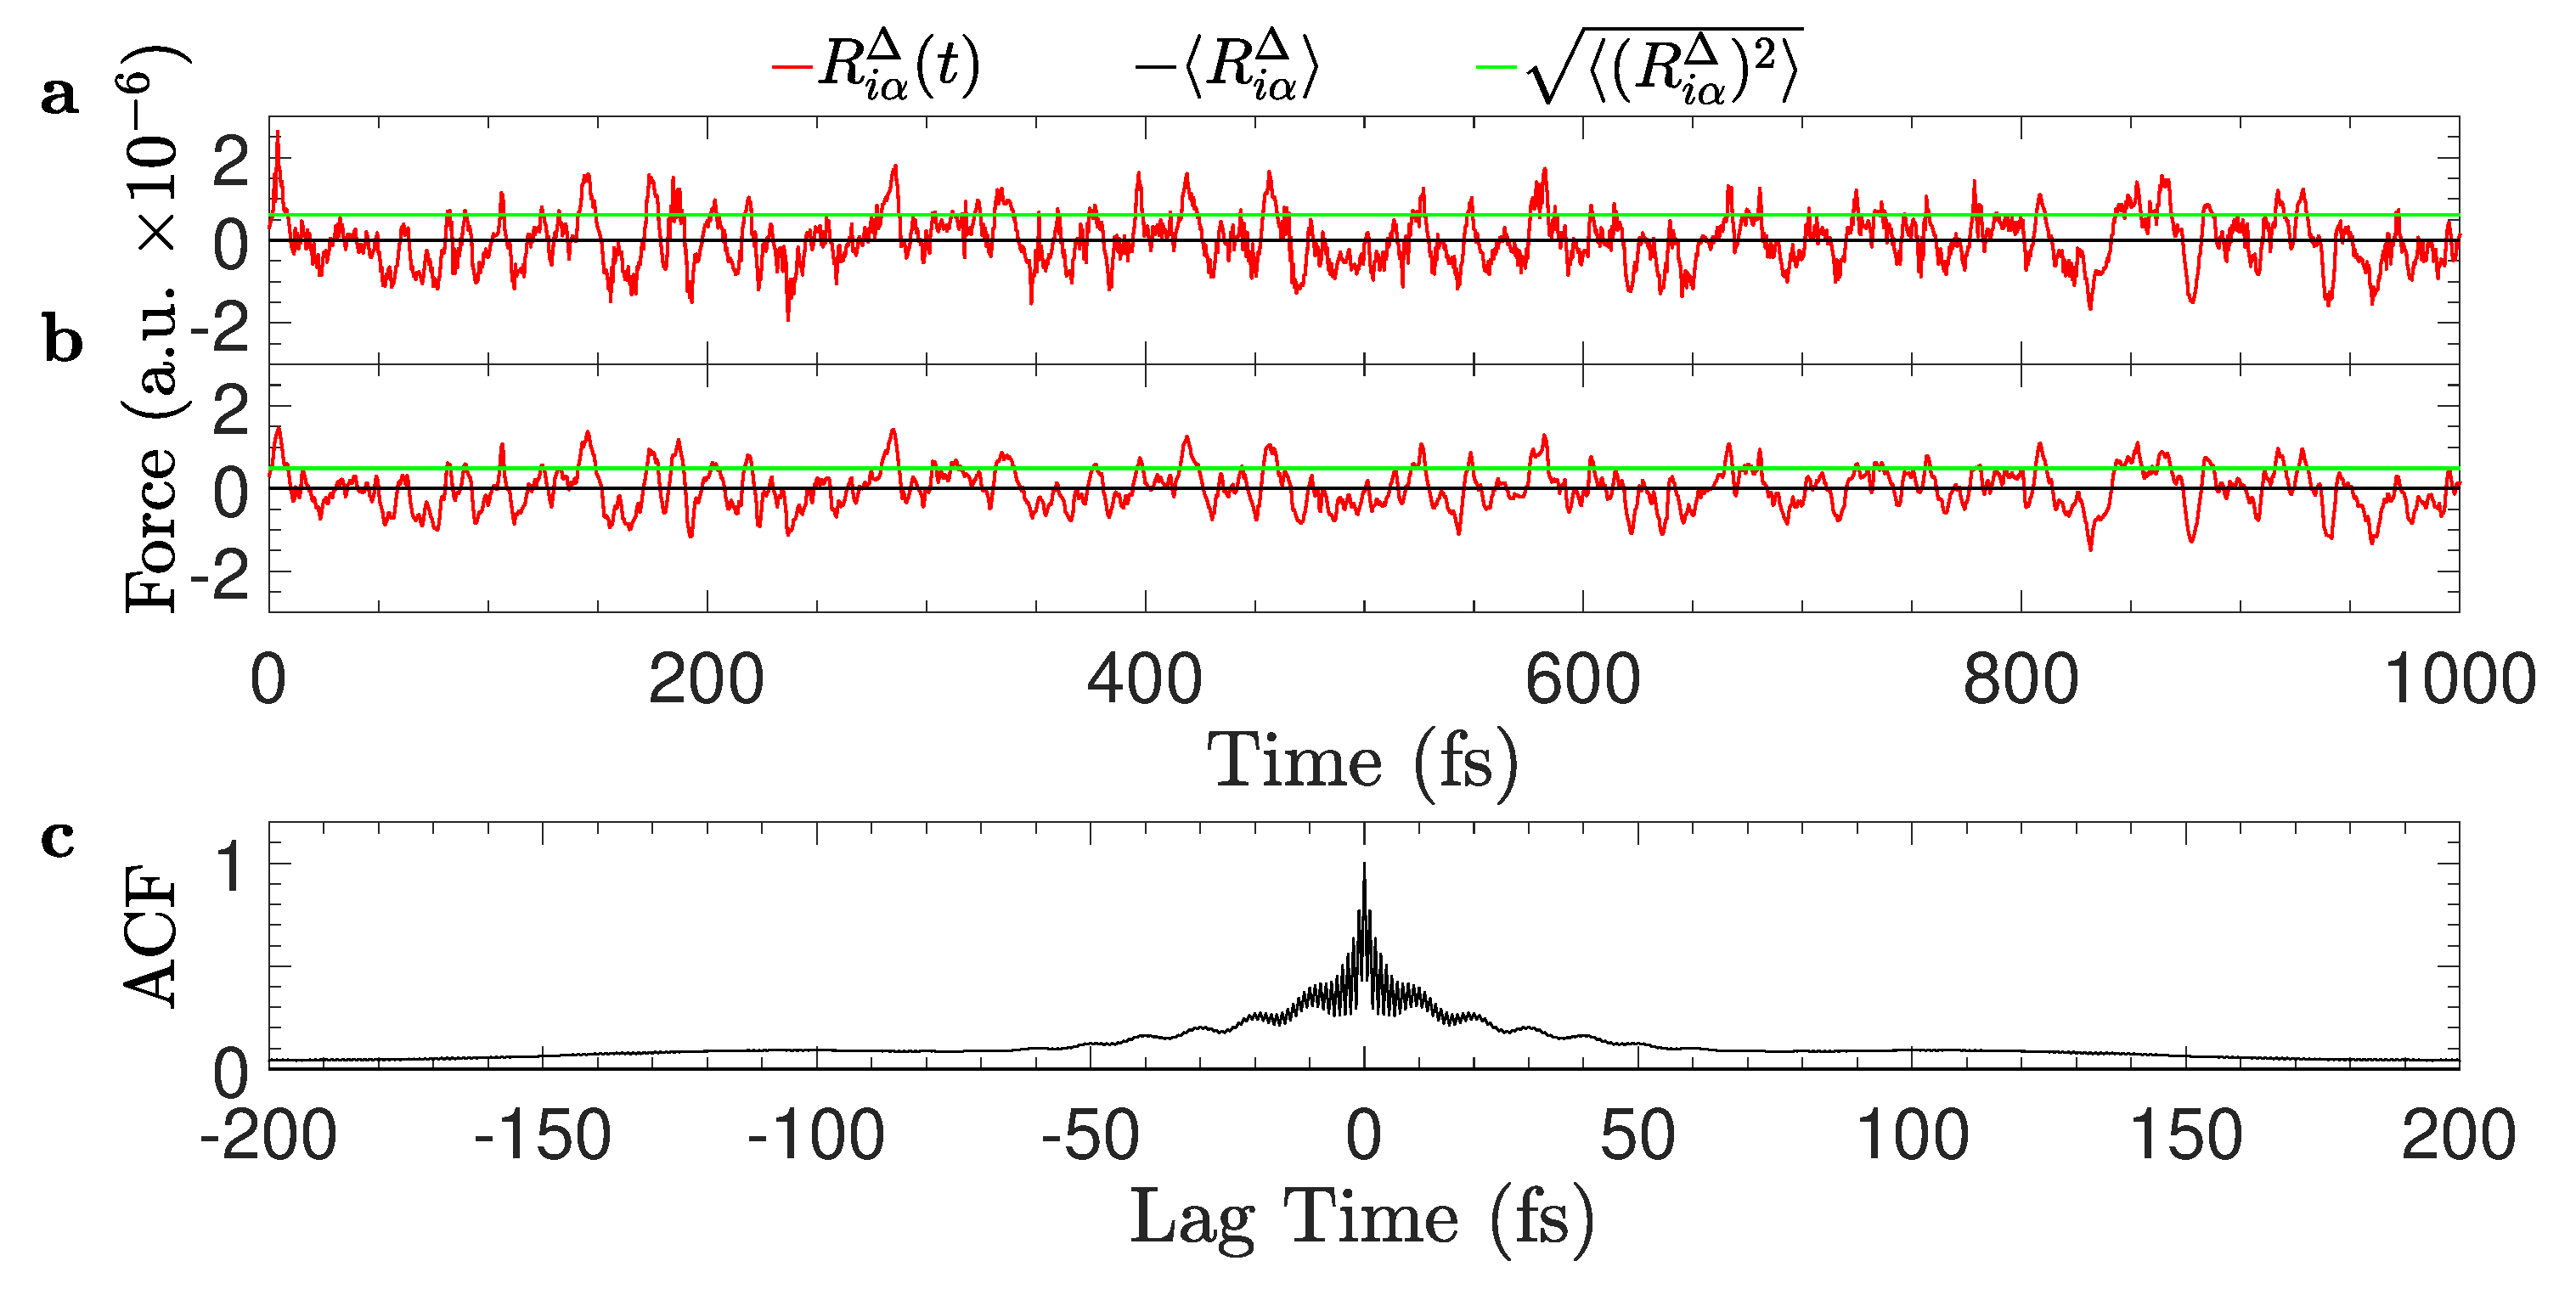
\includegraphics[trim={0.6cm 0.7cm 0.7cm 0.3cm},clip,width=8.6cm]{DeltaForceComparison_with_ACF.eps}
\caption{\label{fig:randomforce}The ``Random force'' along a water molecule dimension $\langle R^{\Delta}_{i\alpha} \rangle (t)$ calculated as the difference between the fully converged Born-Oppenheimer forces and ALMO DFT forces. Here it is clear that Eq.\ (\ref{eq:stochastic2}) is satisfied. 
(a) Plot of $\langle R^{\Delta}_{i\alpha} \rangle (t)$ as a function of time, where $R_{C} = 1.6$ VdWR and $\epsilon_{SCF} = 10^{-2}$.
(b) Plot of $\langle R^{\Delta}_{i\alpha} \rangle (t)$ as a function of time, where $R_{C} = 1.6$ VdWR and forces are fully converged.
(c) Autocorrelation function of plot a, $\langle R^{\Delta}_{i\alpha} (t) R^{\Delta}_{i\alpha} (t+\tau) \rangle $.
Using Eq.\ \ref{eq:delta}, we calculated $\Delta \approx \SI{2e-5}{\per\fs}$, but its true value is $\SI{6e-5}{\per\fs}$ for this system.
Note that the  ACF is not truly a delta-function, and is characterized by rapidly oscillating correlations for short lag times. 
The high frequency correlations made integration of the ACF inaccurate, but provided a decent starting point for further investigation.
The autocorrelation decays rapidly enough that these forces can be considered random and uncorrelated to a good approximation for sufficiently long time scales ($\gg\SI{300}{\fs}$ for this system). 
Calculations were performed with the PBE $\mathrm{E_{XC}}$ functional and the TZV2P basis set on 125 water molecules for 10 ps.}
\end{figure}

\section{Implementation}

The methods presented here are built into CP2K, an open source MD simulation package.~\cite{www:cp2k} 
The computation scheme used is mostly identical to that described in the implementation section of ref.\ \citenum{a:almo-ls}. 
For the dynamical properties calculations using ALMO DFT calculation methods, a periodic cell containing 125 water molecules was simulated for $\SI{10}{\ps}$ at a temperature of $\SI{293}{\K}$ and a constant density of $\SI{1.00597}{\g\per\cm^{3}}$. 
The system was thermostated using the Langevin ensemble (eq.\ \ref{eq:langevin2}) where $\gamma_L$ was set to $\SI{e-3}{\per\fs}$, and $\Delta$ was optimized to the order of $10^{-5}\, \mathrm{fs^{-1}}$. 
Note that for timing benchmarks, $\Delta$ was not optimized. 
This does not have a perceptible effect on calculation time.

Simulations for timing benchmarks were run for ten time steps, which is sufficient for convergence of wavefunctions from an initial guess.
The TZV2P basis set was used to represent MOs, and a cutoff of $\SI{320}{Ry}$ used to represent electron density. 
The exchange-correlation energy was approximated using the PBE functional, which expands upon the local density approximation by considering derivatives of the electron density at each point.~\cite{a:PBEfunctional} 

The reference PES was calculated using the orbital transformation (OT) method~\cite{a:ot,a:ot2} and the Langevin thermostat with $\gamma_L = \SI{e-3}{\per\fs}$. 
All other system parameters were set identical to the ALMO system.

IR spectra, radial distribution functions, diffusivity plots, and diffusion constants were calculated using the open source trajectory analyzer program TRAVIS.~\cite{a:travis-main,a:travis-ir1,a:travis-ir2}

\section{Accuracy}

In order to confirm that ALMO DFT forces are accurate in the limit where localization radius $R_{c} = \infty$, we computed the average difference in force between fully converged Born-Oppenheimer forces and forces calculated from ALMO DFT with varying $R_{c}$. Figure \ref{fig:forcecomp} shows that as $R_{c}$ is increased to infinity, forces converge toward the Born-Oppenheimer limit.

\begin{figure}
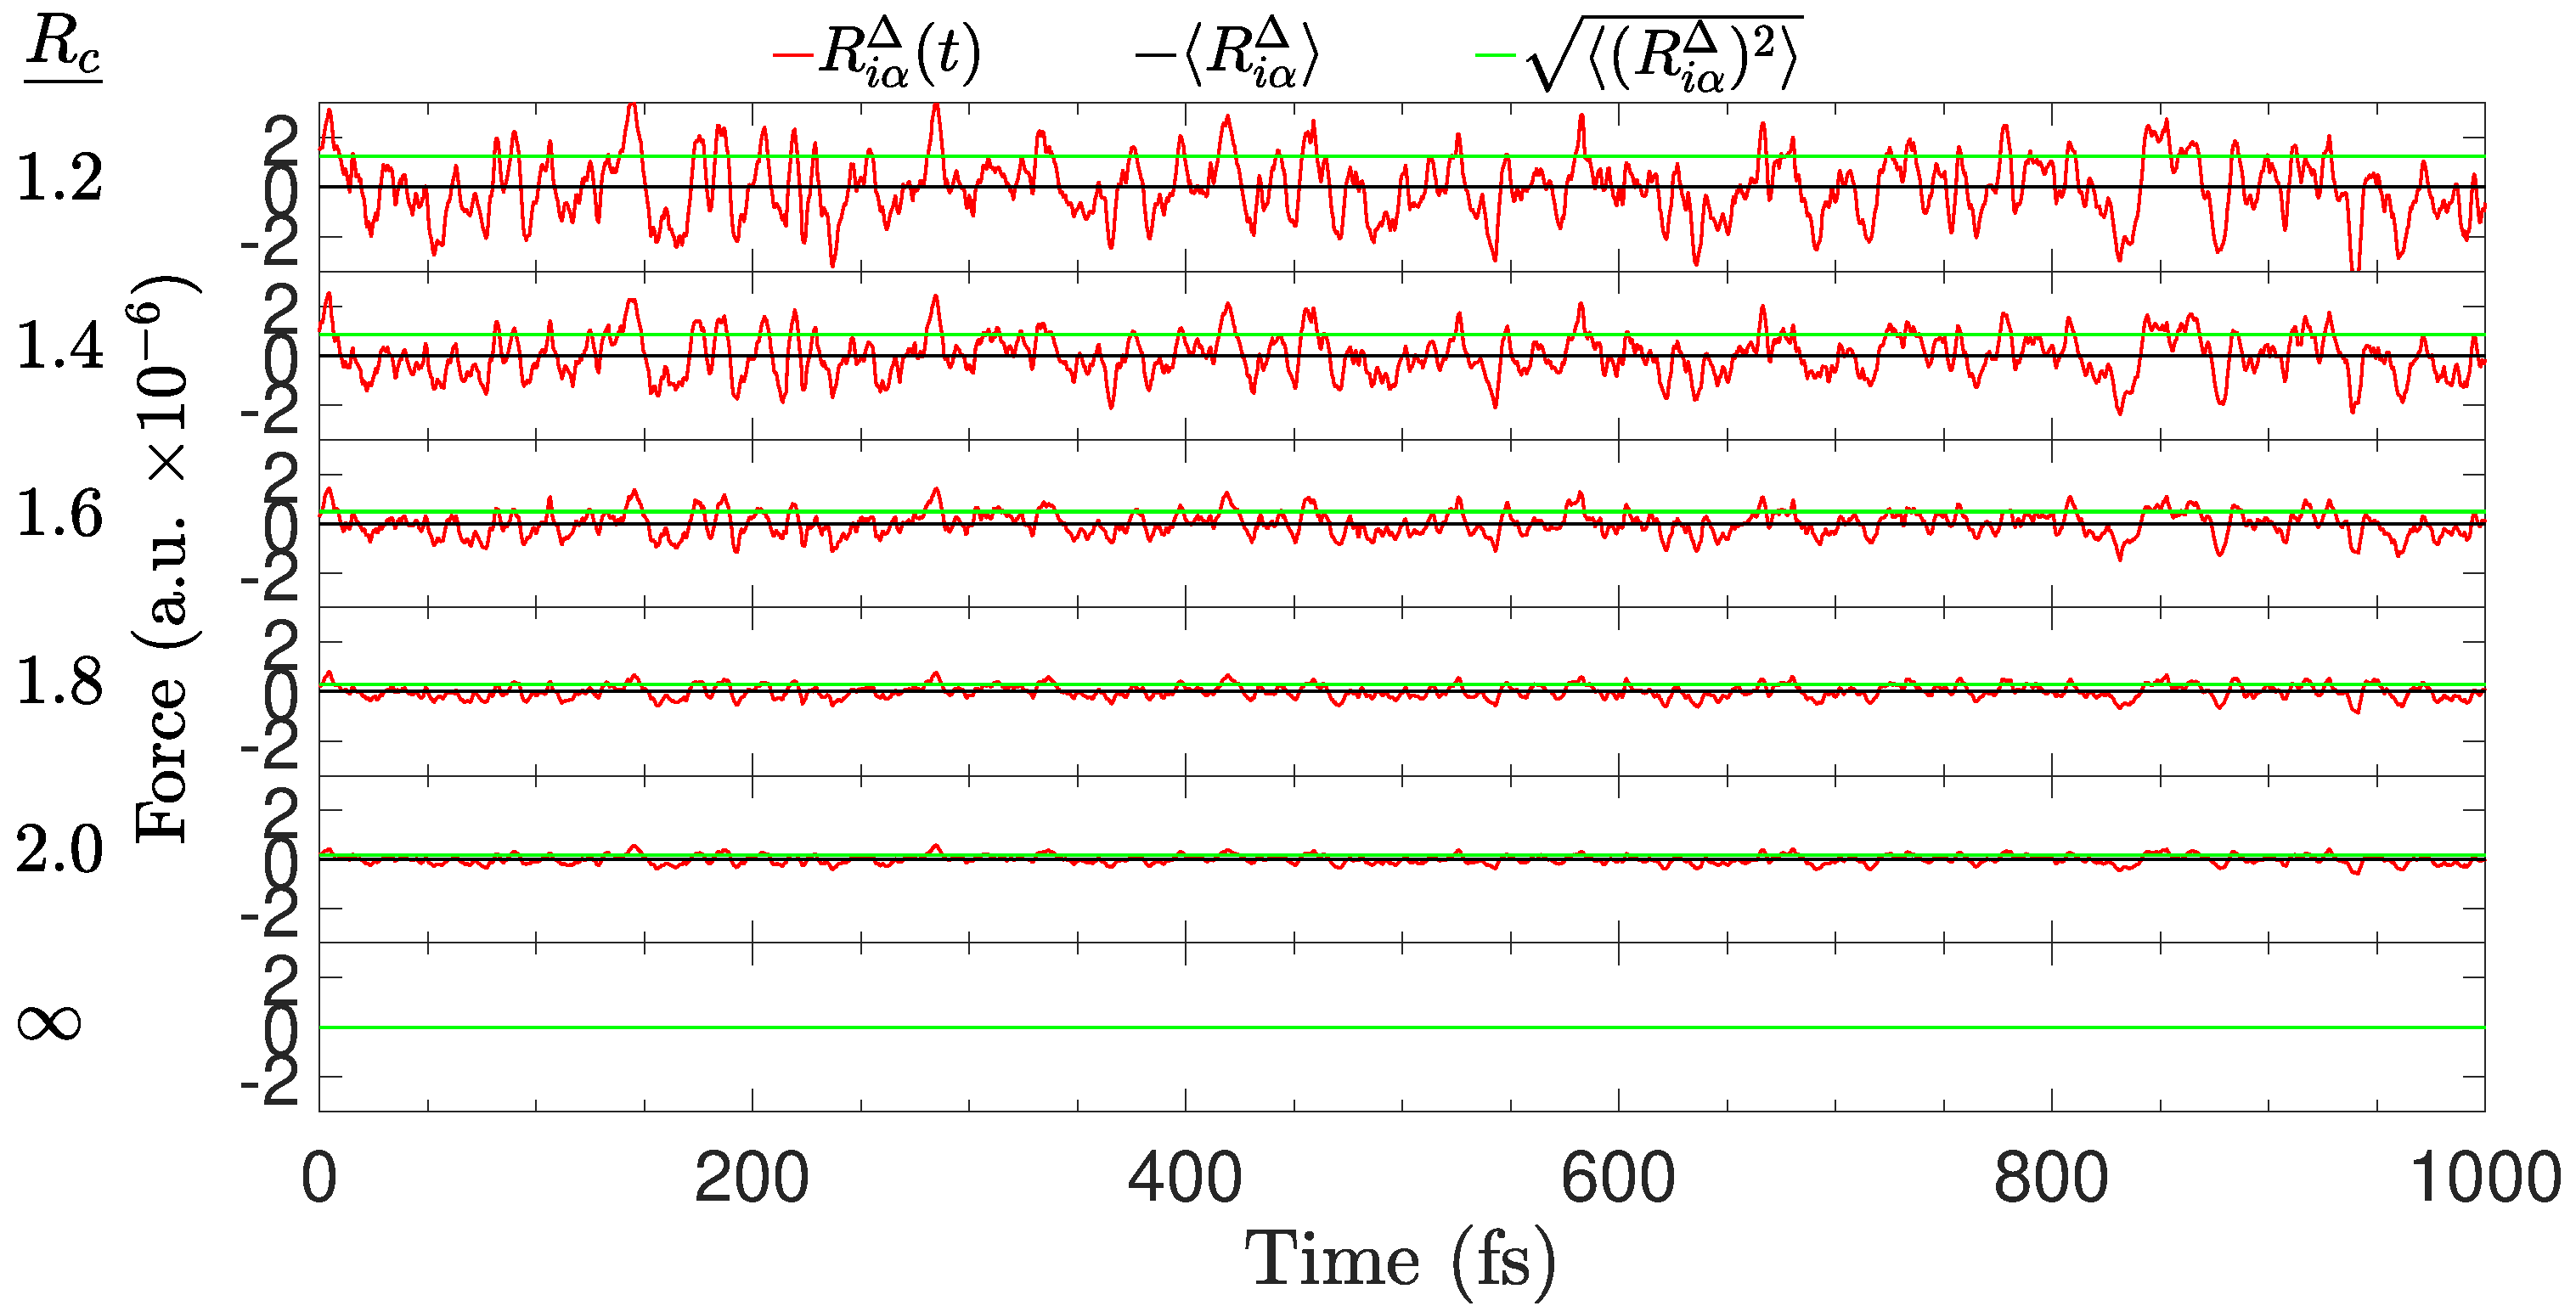
\includegraphics[trim={0.1cm 0cm 0.2cm 0.1cm},clip,width=8.6cm]{DeltaForceComparison_ALMO_SCF.eps}
\caption{\label{fig:forcecomp}The ``Random force'' $\langle R^{\Delta}_{i\alpha} \rangle (t)$ calculated as the average difference between fully converged Born-Oppenheimer forces and fully converged ALMO DFT forces, averaged across all dimensions and all molecules separately at each time step. 
Plotted are the random forces with varying localization radius $R_{c}$, in units of Van der Waals Radii.
Here it is clear that ALMO DFT forces converge to Born-Oppenheimer forces in the limit of $R_{c} \rightarrow \infty$.
Calculations were performed with the PBE $\mathrm{E_{XC}}$ functional and the TZV2P basis set on 125 water molecules for 10 ps.}
\end{figure}

To test the accuracy of ALMO DFT based MD we computed the Infrared (IR) spectrum, radial distribution function (RDF), kinetic energy distribution, and mean-squared displacement (MSD) function from a 10 ps MD trajectory. 
We compared the IR spectrum, RDF, and MSD to equivalent functions calculated from fully converged Kohn-Sham DFT forces (see fig. \ref{fig:dynproperties} and supporting information).
From the MSD functions we also calculated diffusion constants for water at approximately 300 K.
With fully converged forces we calculated D = $\SI{5.47e-9}{\m^{2}\per\s}$.
With ALMO unconverged forces we calculated D = $\SI{5.55E-09}{\m^{2}\per\s}$.


\begin{figure}
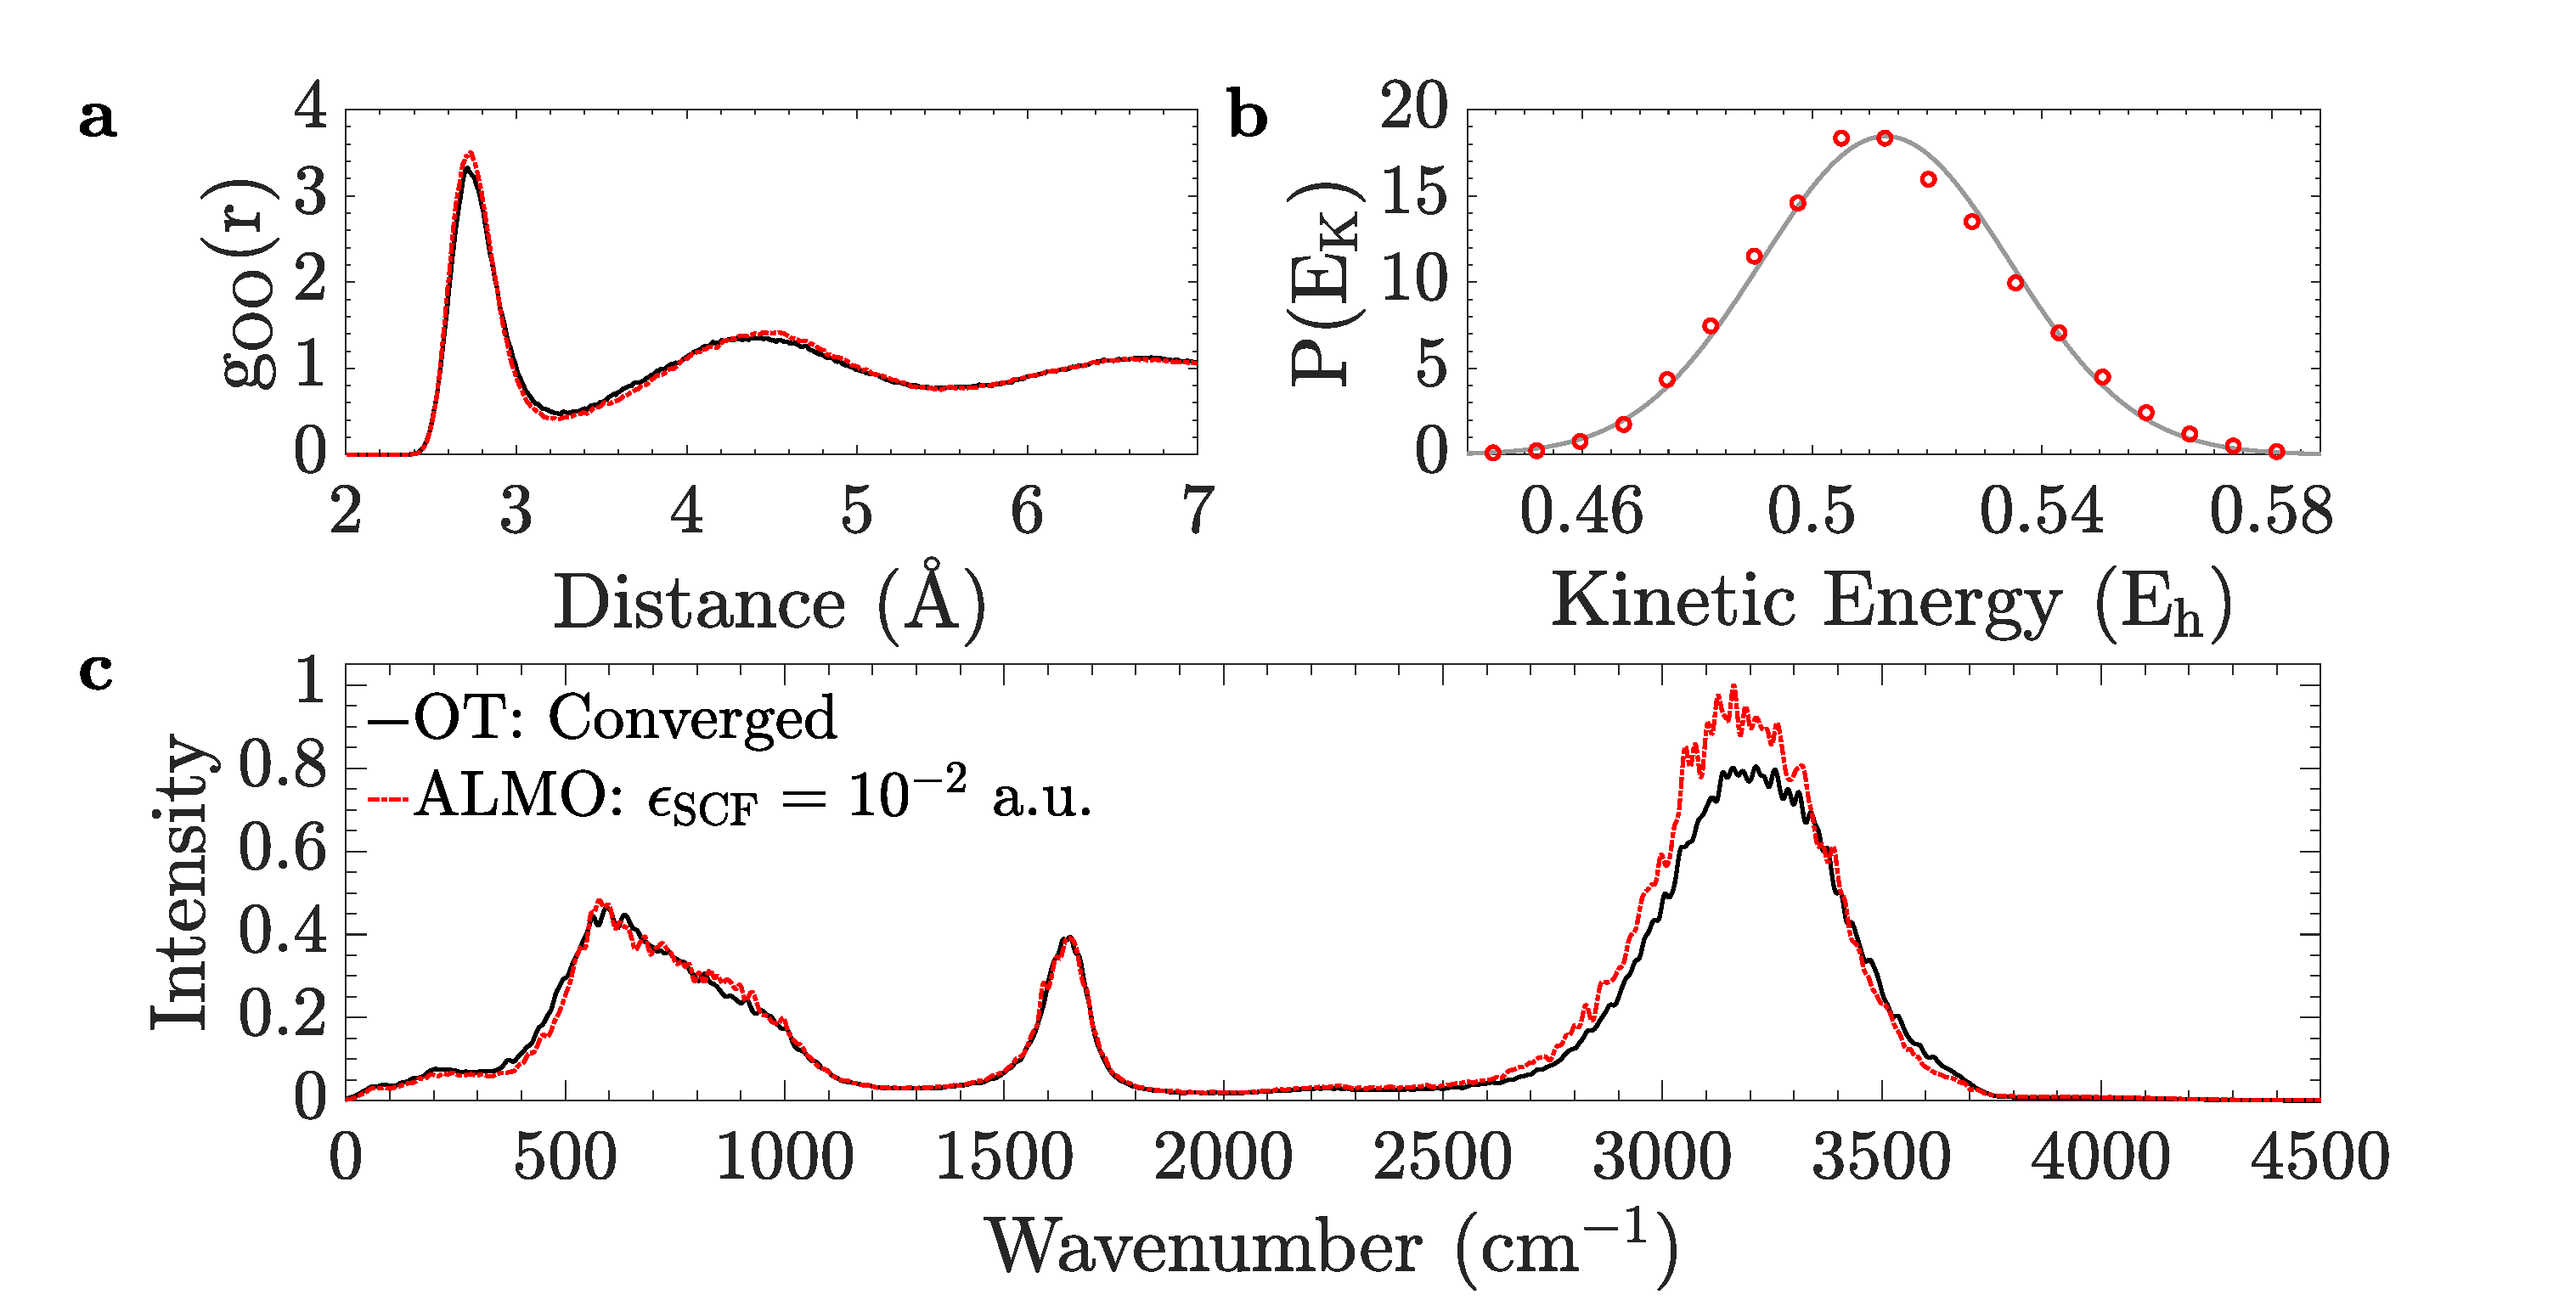
\includegraphics[trim={1.3cm 0.1cm 3.3cm 1.3cm},clip,width=8.6cm]{Dynamical_Data_Tiled.eps}
\caption{\label{fig:dynproperties} Calculated dynamic and static properties of water using ALMO DFT with $\epsilon_{SCF} = 10^{-2}$ and $R_{c} = 1.6$ VdWR.
(a) Radial distribution function of an ALMO simulation compared to OT SCF with fully converged PES. 
(b) Kinetic Energy distribution of an ALMO simulation compared to the theoretical Maxwell-Boltzmann kinetic energy distribution.
(c) Calculated Infrared spectrum of an ALMO simulation compared to OT SCF with fully converged PES.
Calculations were performed with the PBE $\mathrm{E_{XC}}$ functional and TZV2P basis set, using 125 water molecules for 10 ps.}
\end{figure}



\section{Speed}

To show the computational efficiency gained by using unconverged ALMO DFT forces, we compare the average wall-time per MD step over 10 time steps for various values of $\epsilon_{SCF}$ in figure \ref{fig:strongscaling_log}.
For these simulations, we chose to set the localization radius to 1.6 Van der Waal Radii (VdWR), as was done for calculation of dynamical properties.
We also show timing of the fully converged OT SCF method, as well as the recently developed ``second generation Car-Parinello'' SCF method using OT, which improves upon the OT computational cost prefactor.~\cite{a:2ndcpmd}
ALMO methods show excellent LS behavior for all values of $\epsilon_{SCF}$ tested.
OT SCF scales approximately cubically, as expected.
Our findings show that the fastest ALMO SCF method presented here runs faster than second-generation Car-Parinello using OT SCF for water simulations larger than 256 molecules.

Figure \ref{fig:weakscaling} shows that ALMO MD code is well optimized for parallelization, and that computational cost grows linearly under a wide range of available computing power. 
In fact, we were able to successfully simulate systems as large as 32768 water molecules within 25 minutes of wall-clock time using 4096 cores.


%\begin{figure}
%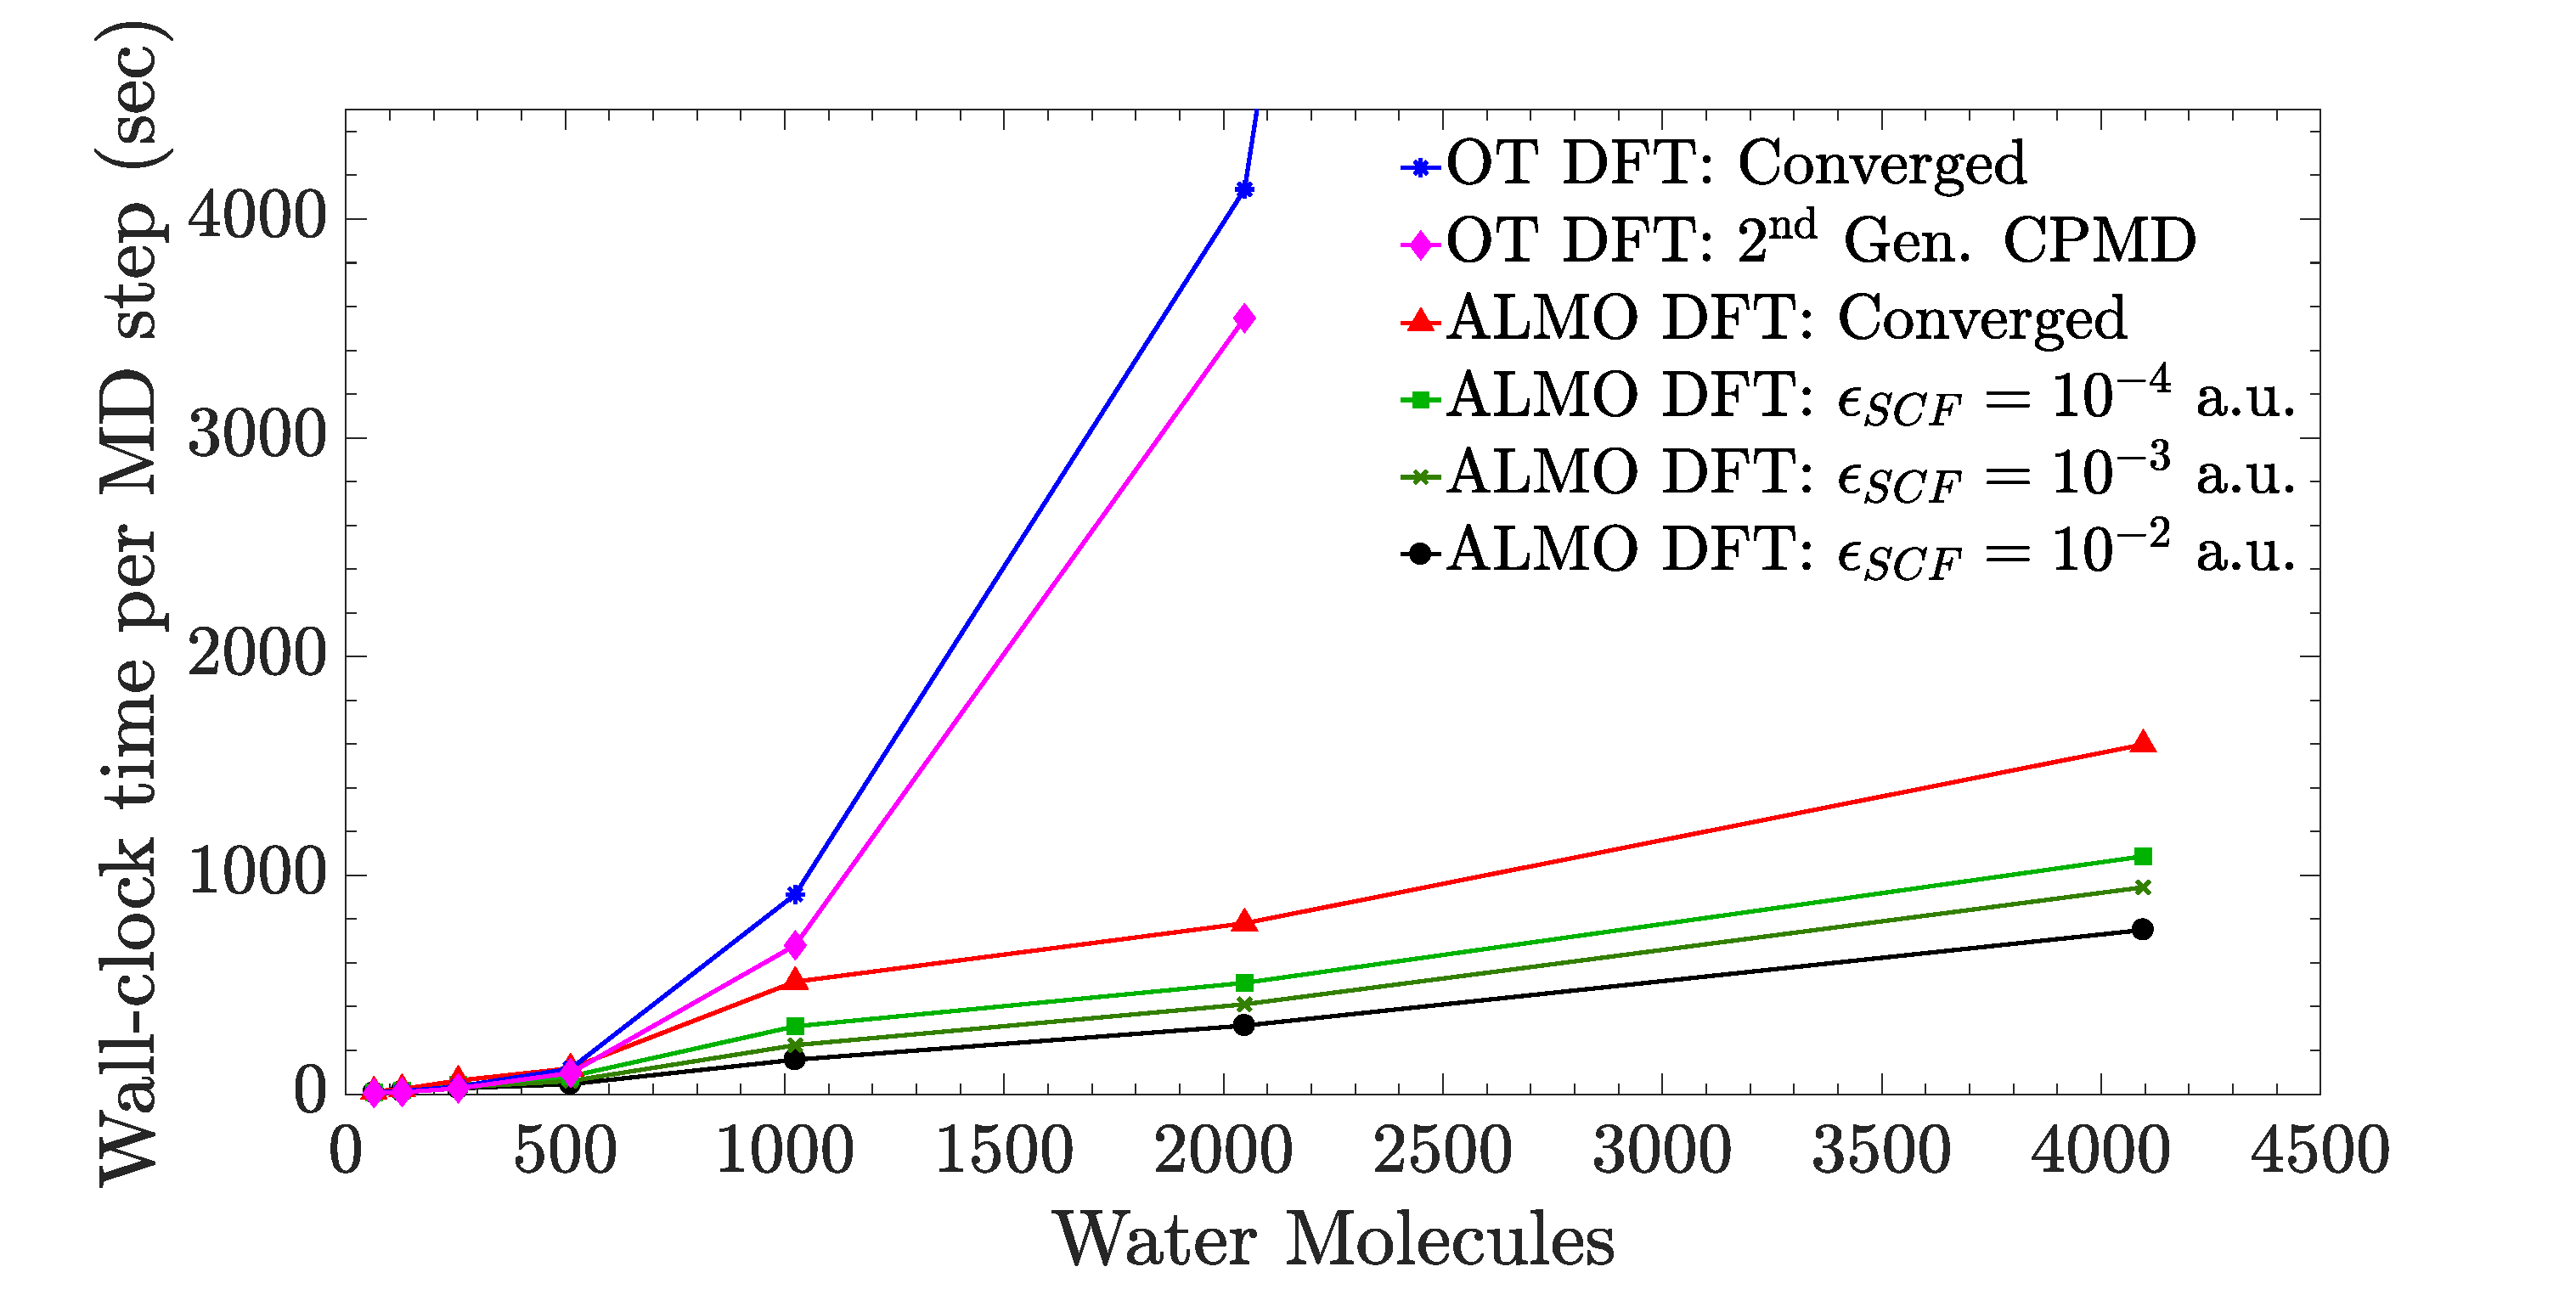
\includegraphics[trim={1.7cm 0.5cm 3.3cm 0.1cm},clip,width=8.6cm]{strongscaling_linear.eps}
%\caption{\label{fig:strongscaling_linear} Linear plots showing LS behaviour of all ALMO methods for liquid water at 298 K. 
%Calculations were performed with the PBE $\mathrm{E_{XC}}$ functional and TZV2P basis set on 256 CPUs. 
%The localization radius was set to $R_{c} = 1.6$ VdWR.}
%\end{figure}

\begin{figure}
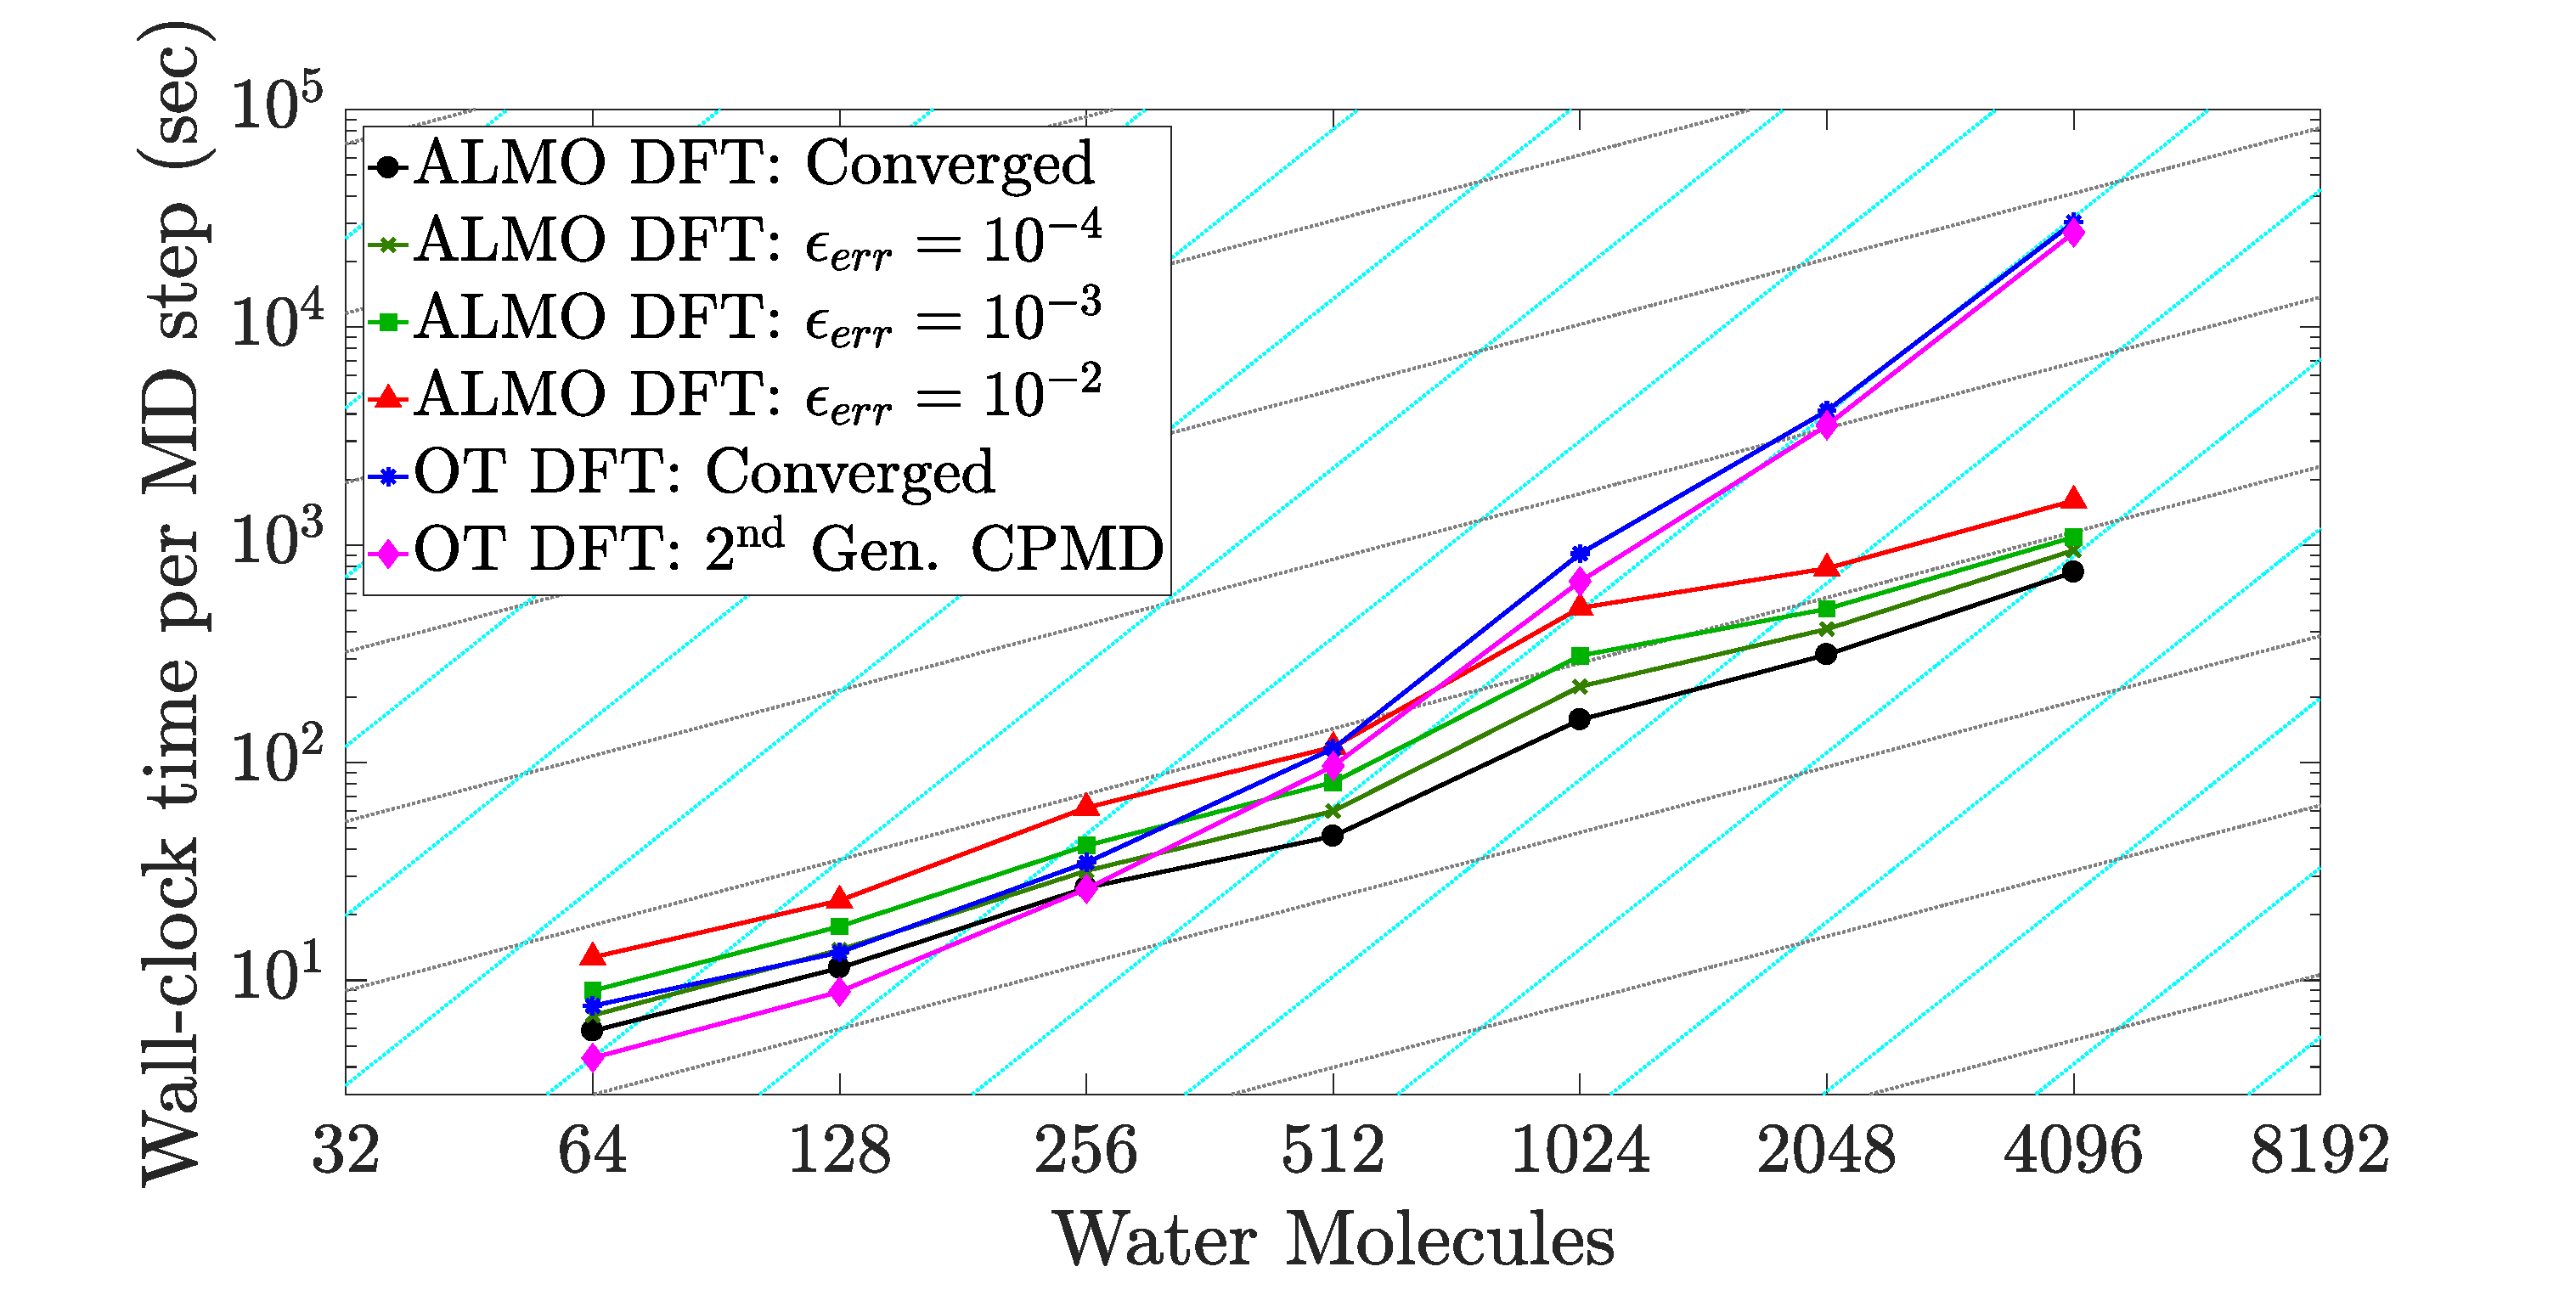
\includegraphics[trim={2.5cm 0.5cm 3.4cm 0.1cm},clip,width=8.6cm]{strongscaling_log.eps}
\caption{\label{fig:strongscaling_log} Logscale plots which show the asymptotic LS behaviour of ALMO methods for liquid water at 298 K.
Compared with the orbital transformation using fully converged SCF and second generation Car-Parinello force calculation methods.
Cyan lines represent perfect cubic scaling, whereas gray lines represent perfect linear scaling. 
Calculations were performed with the PBE $\mathrm{E_{XC}}$ functional and TZV2P basis set on 256 CPUs, averaged over 10 MD steps. 
The localization radius was set to $R_{c} = 1.6$ VdWR.}
\end{figure}


\begin{figure}
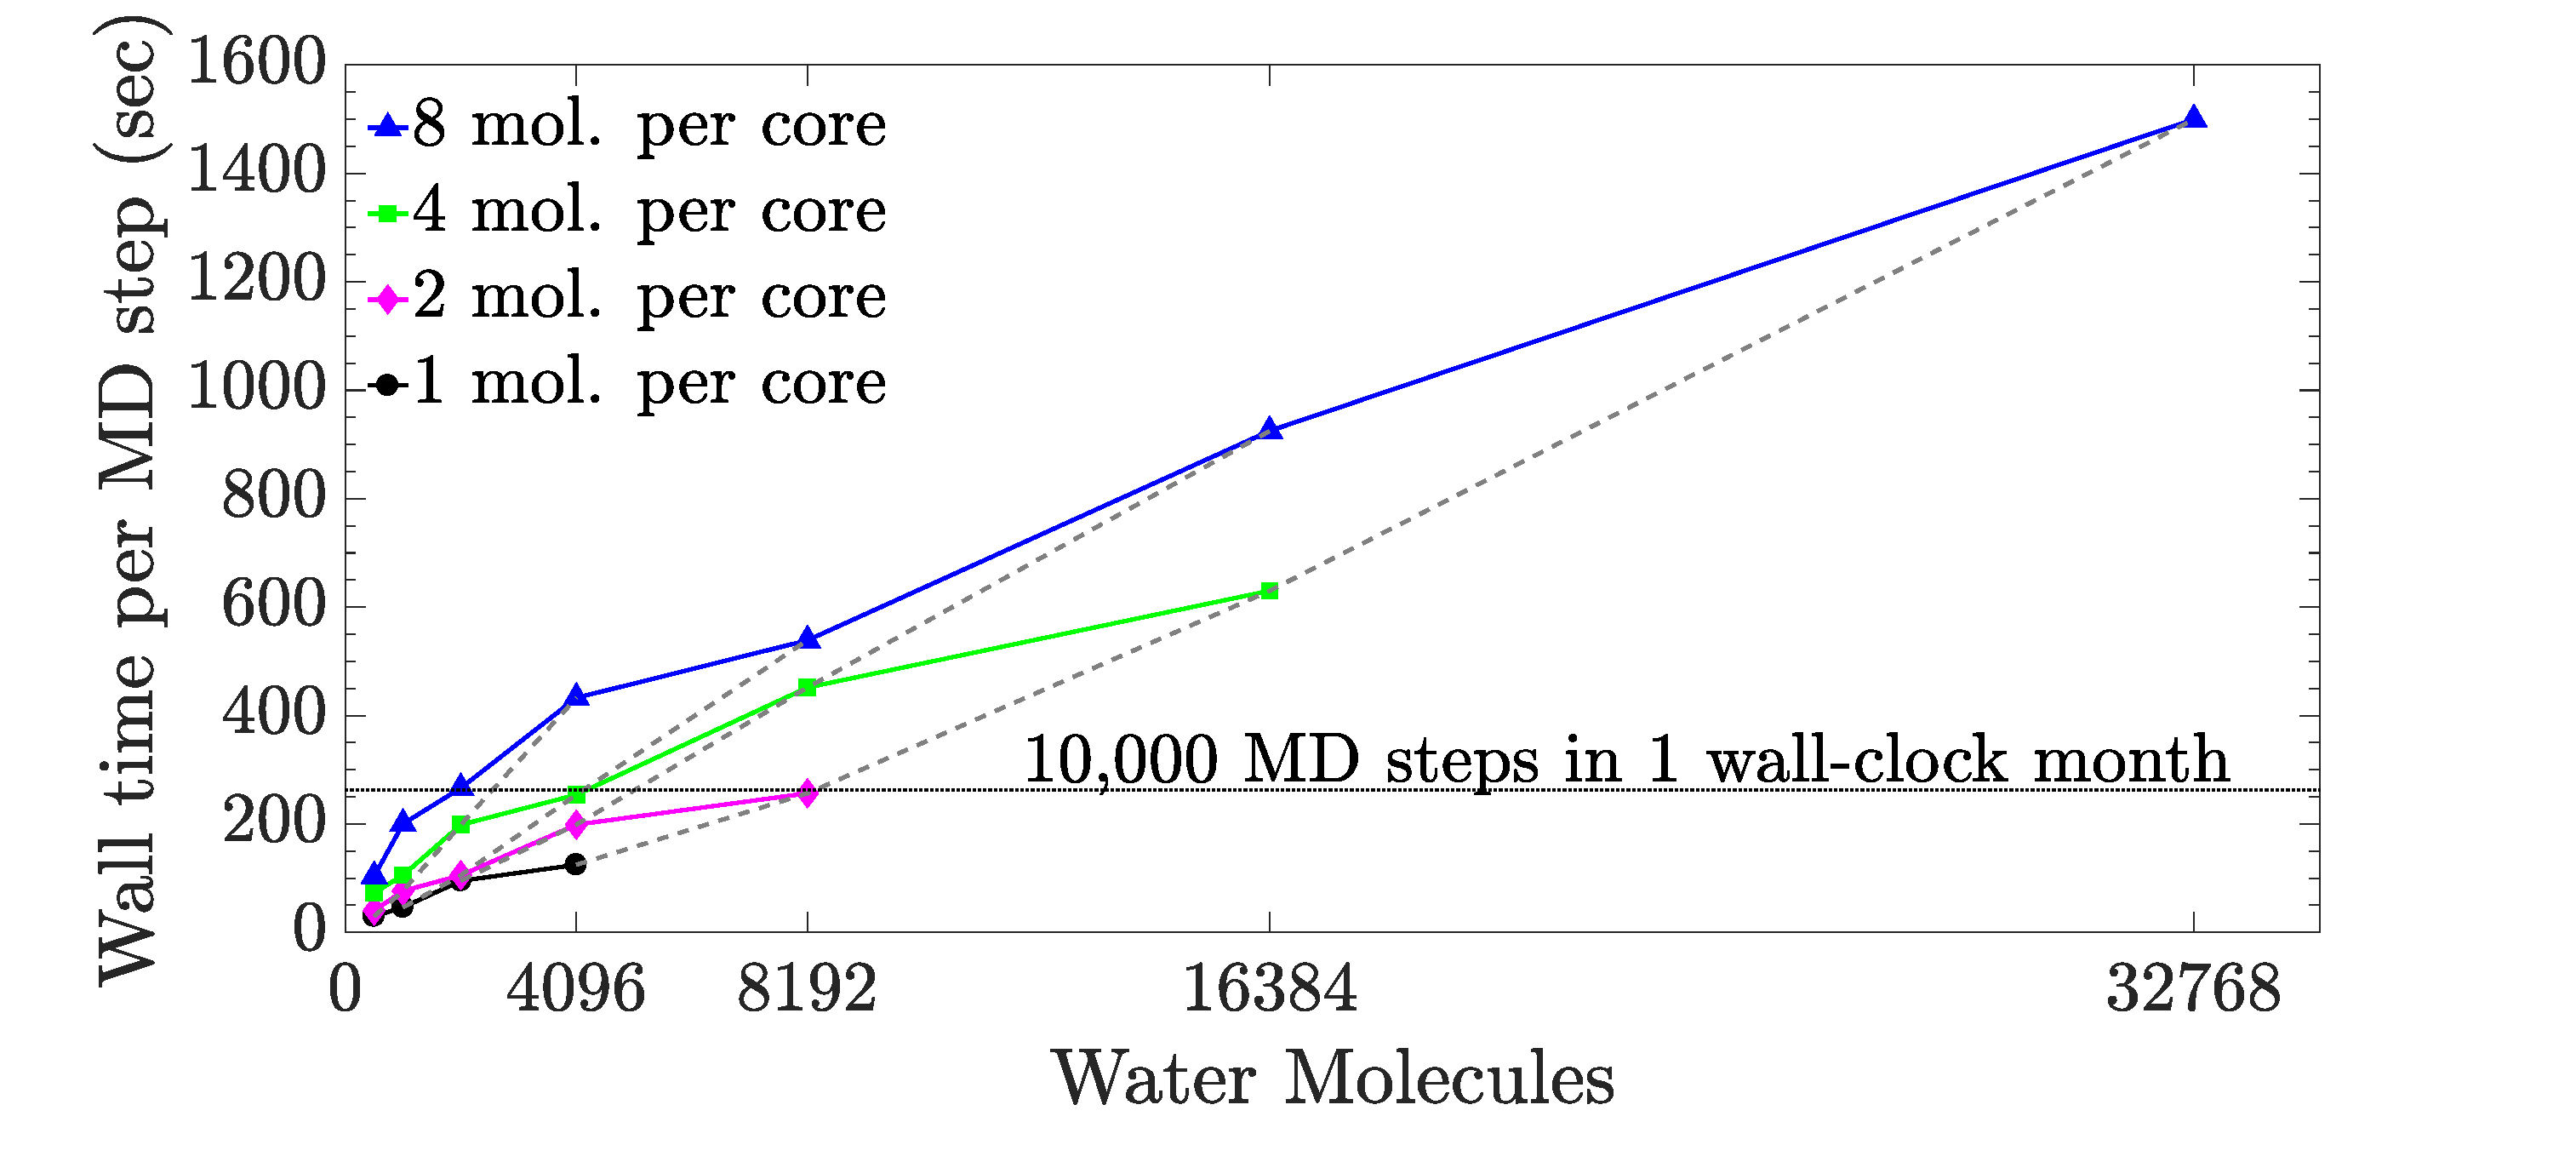
\includegraphics[trim={1.6cm 0cm 4.7cm 0cm},clip,width=8.6cm]{weakscaling.eps}
\caption{\label{fig:weakscaling} Weak scalability benchmarks which show optimization of code for parallel computing.
Dashed gray lines connect systems simulated using the same number of CPU cores, showing LS behaviour over a range of configurations.
Of note is the 32768 molecule system successfully simulated using 4096 cores at around 25 minutes per MD step.
We also show that systems as large as 8192 molecules can be simulated for 10,000 MD steps in under a month using our method.
Calculations were performed with the PBE $\mathrm{E_{XC}}$ functional and TZV2P basis set, averaged over 10 MD steps. 
The localization radius was set to $R_{c} = 1.6$ VdWR and $\epsilon_{SCF} = 10^{-2}$.}
\end{figure}


\section{Conclusions} 

\textbf{Acknowledgments.} The research was funded by the Natural Sciences and Engineering Research Council of Canada through the Discovery Grant. The authors are grateful to Compute Canada and McGill HPC Centre for computer time.

%\textbf{Supporting Information}
%Calculated radial distribution functions of liquid water, comparison of timing benchmarks for the DZVP and TZV2P basis sets, timing benchmarks for systems containing 32,768 water molecules, timing benchmarks for the Kohn-Sham matrix build. This material is available free of charge via the Internet at http://pubs.acs.org.

\bibliography{almo-langevin}

\end{document}
